\documentclass[11pt]{article}
%\usepackage{psfig}
\usepackage{latexsym}
\usepackage{amsfonts}
\usepackage{hyperref}
\usepackage{url}
\usepackage{listings}
% to use hyperlinks in References section
\hypersetup{urlbordercolor={1 1 1}}
\usepackage{graphicx}
\usepackage{listings}

%define colors
\usepackage{xcolor}
\definecolor{dkgreen}{rgb}{0,0.6,0}
\definecolor{gray}{rgb}{0.5,0.5,0.5}
\definecolor{mauve}{rgb}{0.58,0,0.82}
\usepackage{graphicx}
\usepackage{hyperref}
\hypersetup{urlbordercolor={1 1 1}}
\DeclareGraphicsExtensions{.pdf,.jpg,.png,.eps}
\setlength{\textheight}{8.5in}
\setlength{\textwidth}{6.0in}
\setlength{\headheight}{0in}
\addtolength{\topmargin}{-.5in}
\addtolength{\oddsidemargin}{-.5in}


\newenvironment{cvl}{\begin{list}{$\bullet$}{
\setlength{\leftmargin}{0.3in} \setlength{\labelsep}{0.07in}
\setlength{\labelwidth}{0.17in} \setlength{\rightmargin}{0.0in}
\setlength{\topsep}{0.000in} \setlength{\partopsep}{0.000in}
\setlength{\parskip}{0.000in} \setlength{\parsep}{0.005in}
\setlength{\itemsep}{0.005in}}}{\end{list}}

\DeclareGraphicsExtensions{.pdf,.jpg,.png,.eps}
\usepackage[T1]{fontenc}   %special characters copy-able

% \usepackage{times}
\usepackage{enumerate}

\usepackage{courier}
\usepackage{amsmath}
\usepackage{amssymb}
\usepackage{upgreek}

%--------------
%% Modified by Zhiqiang Lin
%% 01/18/2012
%%
%% Template file was from http://www.cs.umd.edu/~jkatz
%%
%% preamble.tex
%% this should be included with a command like
%% %--------------
%% Modified by Zhiqiang Lin
%% 01/18/2012
%%
%% Template file was from http://www.cs.umd.edu/~jkatz
%%
%% preamble.tex
%% this should be included with a command like
%% %--------------
%% Modified by Zhiqiang Lin
%% 01/18/2012
%%
%% Template file was from http://www.cs.umd.edu/~jkatz
%%
%% preamble.tex
%% this should be included with a command like
%% \input{preamble.tex}
%% \lecture{``lecture number''}{``date''}{``name of professor''}{``name
%%  of student''}

\hbadness=10000
\vbadness=10000

\newcommand{\handout}[5]{
   \renewcommand{\thepage}{#1-\arabic{page}}
   \noindent
   \begin{center}
   \framebox{
      \vbox{
    \hbox to 5.78in { {\bf CSE 5473 --- Network Security} 
     	 \hfill #2 }
       \vspace{4mm}
       \hbox to 5.78in { {\Large \hfill #5  \hfill} }
       \vspace{2mm}
       \hbox to 5.78in { {\it #3 \hfill #4} }
      }
   }
   \end{center}
   \vspace*{4mm}
}

\newcommand{\lecture}[4]{\handout{#1}{#2}{#3}{#4}{#1}}
%\newcommand{\lecture}[4]{\handout{#1}{#2}{Lecturer: #3}{Scribe(s): #4}{Lecture #1}}

\def\epsilon{\varepsilon}
\def\phi{\varphi}
\def\bool{\{0,1\}}
\def\poly{{\sf poly}}
\def\cross{\times}

\newcommand{\xor}{\oplus}
\newcommand{\Xor}{\bigoplus}
\newcommand{\ceil}[1]{\left\lceil {#1} \right\rceil}
\newcommand{\floor}[1]{\left\lfloor #1 \right\rfloor}
\newcommand{\ignore}[1]{}
\newcommand{\integers}[1]{{\mathbb Z}_{#1}}
\newcommand{\bydef}{\stackrel{\rm def}{=}}
\newcommand{\isequal}{\stackrel{\rm ?}{=}}
\newcommand{\compeq}{\stackrel{\rm c}{\equiv}} % computationally indistinguishable

\newcommand{\qed}{\hspace*{\fill}\rule{7pt}{7pt}}
\newenvironment{proof_sketch}{\noindent{\bf Sketch of Proof} (Informal)\hspace*{1em}}{\qed\medskip}
\newenvironment{proof}{\noindent{\bf Proof}\hspace*{1em}}{\qed\medskip}
\newenvironment{proofof}[1]{\noindent{\bf Proof} of #1:\hspace*{1em}}{\qed\medskip}
%\newenvironment{claim}{\noindent{\bf Claim}\hspace*{1em}\begin{em}}{\end{em}\medskip}
\newcounter{defcounter}
\setcounter{defcounter}{1}
\newenvironment{definition}{\medskip\noindent{\bf Definition \thedefcounter}}{\hspace*{\fill}$\diamondsuit$\stepcounter{defcounter}\medskip}
\newtheorem{theorem}{Theorem}
\newtheorem{corollary}[theorem]{Corollary}
\newtheorem{lemma}[theorem]{Lemma}
\newtheorem{claim}[theorem]{Claim}
\newtheorem{fact}[theorem]{Fact}
\newtheorem{conjecture}[theorem]{Conjecture}
\newenvironment{assumption}{\noindent{\bf Assumption}\hspace*{1em}\begin{em}}{\end{em}\medskip}
\newenvironment{remark}{\noindent{\bf Remark}\hspace*{1em}}{\bigskip}

\ignore{
\newcommand{\FOR}{{\bf for}}
\newcommand{\TO}{{\bf to}}
\newcommand{\DO}{{\bf do}}
\newcommand{\WHILE}{{\bf while}}
\newcommand{\AND}{{\bf and}}
\newcommand{\IF}{{\bf if}}
\newcommand{\THEN}{{\bf then}}
\newcommand{\ELSE}{{\bf else}}

%%% You probably will not need to use the commands listed below

\makeatletter
\def\fnum@figure{{\bf Figure \thefigure}}
\def\fnum@table{{\bf Table \thetable}}
\long\def\@mycaption#1[#2]#3{\addcontentsline{\csname
  ext@#1\endcsname}{#1}{\protect\numberline{\csname 
  the#1\endcsname}{\ignorespaces #2}}\par
  \begingroup
    \@parboxrestore
    \small
    \@makecaption{\csname fnum@#1\endcsname}{\ignorespaces #3}\par
  \endgroup}
\def\mycaption{\refstepcounter\@captype \@dblarg{\@mycaption\@captype}}
\makeatother

\newcommand{\figcaption}[1]{\mycaption[]{#1}}
\newcommand{\tabcaption}[1]{\mycaption[]{#1}}
\newcommand{\head}[1]{\chapter[Lecture \##1]{}}
\newcommand{\mathify}[1]{\ifmmode{#1}\else\mbox{$#1$}\fi}
\def\half{\frac{1}{2}}

\newcommand{\fig}[4]{
        \begin{figure}
        \setlength{\epsfysize}{#2}
        \vspace{3mm}
        \centerline{\epsfbox{#4}}
        \caption{#3} \label{#1}
        \end{figure}
        }
}



%% \lecture{``lecture number''}{``date''}{``name of professor''}{``name
%%  of student''}

\hbadness=10000
\vbadness=10000

\newcommand{\handout}[5]{
   \renewcommand{\thepage}{#1-\arabic{page}}
   \noindent
   \begin{center}
   \framebox{
      \vbox{
    \hbox to 5.78in { {\bf CSE 5473 --- Network Security} 
     	 \hfill #2 }
       \vspace{4mm}
       \hbox to 5.78in { {\Large \hfill #5  \hfill} }
       \vspace{2mm}
       \hbox to 5.78in { {\it #3 \hfill #4} }
      }
   }
   \end{center}
   \vspace*{4mm}
}

\newcommand{\lecture}[4]{\handout{#1}{#2}{#3}{#4}{#1}}
%\newcommand{\lecture}[4]{\handout{#1}{#2}{Lecturer: #3}{Scribe(s): #4}{Lecture #1}}

\def\epsilon{\varepsilon}
\def\phi{\varphi}
\def\bool{\{0,1\}}
\def\poly{{\sf poly}}
\def\cross{\times}

\newcommand{\xor}{\oplus}
\newcommand{\Xor}{\bigoplus}
\newcommand{\ceil}[1]{\left\lceil {#1} \right\rceil}
\newcommand{\floor}[1]{\left\lfloor #1 \right\rfloor}
\newcommand{\ignore}[1]{}
\newcommand{\integers}[1]{{\mathbb Z}_{#1}}
\newcommand{\bydef}{\stackrel{\rm def}{=}}
\newcommand{\isequal}{\stackrel{\rm ?}{=}}
\newcommand{\compeq}{\stackrel{\rm c}{\equiv}} % computationally indistinguishable

\newcommand{\qed}{\hspace*{\fill}\rule{7pt}{7pt}}
\newenvironment{proof_sketch}{\noindent{\bf Sketch of Proof} (Informal)\hspace*{1em}}{\qed\medskip}
\newenvironment{proof}{\noindent{\bf Proof}\hspace*{1em}}{\qed\medskip}
\newenvironment{proofof}[1]{\noindent{\bf Proof} of #1:\hspace*{1em}}{\qed\medskip}
%\newenvironment{claim}{\noindent{\bf Claim}\hspace*{1em}\begin{em}}{\end{em}\medskip}
\newcounter{defcounter}
\setcounter{defcounter}{1}
\newenvironment{definition}{\medskip\noindent{\bf Definition \thedefcounter}}{\hspace*{\fill}$\diamondsuit$\stepcounter{defcounter}\medskip}
\newtheorem{theorem}{Theorem}
\newtheorem{corollary}[theorem]{Corollary}
\newtheorem{lemma}[theorem]{Lemma}
\newtheorem{claim}[theorem]{Claim}
\newtheorem{fact}[theorem]{Fact}
\newtheorem{conjecture}[theorem]{Conjecture}
\newenvironment{assumption}{\noindent{\bf Assumption}\hspace*{1em}\begin{em}}{\end{em}\medskip}
\newenvironment{remark}{\noindent{\bf Remark}\hspace*{1em}}{\bigskip}

\ignore{
\newcommand{\FOR}{{\bf for}}
\newcommand{\TO}{{\bf to}}
\newcommand{\DO}{{\bf do}}
\newcommand{\WHILE}{{\bf while}}
\newcommand{\AND}{{\bf and}}
\newcommand{\IF}{{\bf if}}
\newcommand{\THEN}{{\bf then}}
\newcommand{\ELSE}{{\bf else}}

%%% You probably will not need to use the commands listed below

\makeatletter
\def\fnum@figure{{\bf Figure \thefigure}}
\def\fnum@table{{\bf Table \thetable}}
\long\def\@mycaption#1[#2]#3{\addcontentsline{\csname
  ext@#1\endcsname}{#1}{\protect\numberline{\csname 
  the#1\endcsname}{\ignorespaces #2}}\par
  \begingroup
    \@parboxrestore
    \small
    \@makecaption{\csname fnum@#1\endcsname}{\ignorespaces #3}\par
  \endgroup}
\def\mycaption{\refstepcounter\@captype \@dblarg{\@mycaption\@captype}}
\makeatother

\newcommand{\figcaption}[1]{\mycaption[]{#1}}
\newcommand{\tabcaption}[1]{\mycaption[]{#1}}
\newcommand{\head}[1]{\chapter[Lecture \##1]{}}
\newcommand{\mathify}[1]{\ifmmode{#1}\else\mbox{$#1$}\fi}
\def\half{\frac{1}{2}}

\newcommand{\fig}[4]{
        \begin{figure}
        \setlength{\epsfysize}{#2}
        \vspace{3mm}
        \centerline{\epsfbox{#4}}
        \caption{#3} \label{#1}
        \end{figure}
        }
}



%% \lecture{``lecture number''}{``date''}{``name of professor''}{``name
%%  of student''}

\hbadness=10000
\vbadness=10000

\newcommand{\handout}[5]{
   \renewcommand{\thepage}{#1-\arabic{page}}
   \noindent
   \begin{center}
   \framebox{
      \vbox{
    \hbox to 5.78in { {\bf CSE 5473 --- Network Security} 
     	 \hfill #2 }
       \vspace{4mm}
       \hbox to 5.78in { {\Large \hfill #5  \hfill} }
       \vspace{2mm}
       \hbox to 5.78in { {\it #3 \hfill #4} }
      }
   }
   \end{center}
   \vspace*{4mm}
}

\newcommand{\lecture}[4]{\handout{#1}{#2}{#3}{#4}{#1}}
%\newcommand{\lecture}[4]{\handout{#1}{#2}{Lecturer: #3}{Scribe(s): #4}{Lecture #1}}

\def\epsilon{\varepsilon}
\def\phi{\varphi}
\def\bool{\{0,1\}}
\def\poly{{\sf poly}}
\def\cross{\times}

\newcommand{\xor}{\oplus}
\newcommand{\Xor}{\bigoplus}
\newcommand{\ceil}[1]{\left\lceil {#1} \right\rceil}
\newcommand{\floor}[1]{\left\lfloor #1 \right\rfloor}
\newcommand{\ignore}[1]{}
\newcommand{\integers}[1]{{\mathbb Z}_{#1}}
\newcommand{\bydef}{\stackrel{\rm def}{=}}
\newcommand{\isequal}{\stackrel{\rm ?}{=}}
\newcommand{\compeq}{\stackrel{\rm c}{\equiv}} % computationally indistinguishable

\newcommand{\qed}{\hspace*{\fill}\rule{7pt}{7pt}}
\newenvironment{proof_sketch}{\noindent{\bf Sketch of Proof} (Informal)\hspace*{1em}}{\qed\medskip}
\newenvironment{proof}{\noindent{\bf Proof}\hspace*{1em}}{\qed\medskip}
\newenvironment{proofof}[1]{\noindent{\bf Proof} of #1:\hspace*{1em}}{\qed\medskip}
%\newenvironment{claim}{\noindent{\bf Claim}\hspace*{1em}\begin{em}}{\end{em}\medskip}
\newcounter{defcounter}
\setcounter{defcounter}{1}
\newenvironment{definition}{\medskip\noindent{\bf Definition \thedefcounter}}{\hspace*{\fill}$\diamondsuit$\stepcounter{defcounter}\medskip}
\newtheorem{theorem}{Theorem}
\newtheorem{corollary}[theorem]{Corollary}
\newtheorem{lemma}[theorem]{Lemma}
\newtheorem{claim}[theorem]{Claim}
\newtheorem{fact}[theorem]{Fact}
\newtheorem{conjecture}[theorem]{Conjecture}
\newenvironment{assumption}{\noindent{\bf Assumption}\hspace*{1em}\begin{em}}{\end{em}\medskip}
\newenvironment{remark}{\noindent{\bf Remark}\hspace*{1em}}{\bigskip}

\ignore{
\newcommand{\FOR}{{\bf for}}
\newcommand{\TO}{{\bf to}}
\newcommand{\DO}{{\bf do}}
\newcommand{\WHILE}{{\bf while}}
\newcommand{\AND}{{\bf and}}
\newcommand{\IF}{{\bf if}}
\newcommand{\THEN}{{\bf then}}
\newcommand{\ELSE}{{\bf else}}

%%% You probably will not need to use the commands listed below

\makeatletter
\def\fnum@figure{{\bf Figure \thefigure}}
\def\fnum@table{{\bf Table \thetable}}
\long\def\@mycaption#1[#2]#3{\addcontentsline{\csname
  ext@#1\endcsname}{#1}{\protect\numberline{\csname 
  the#1\endcsname}{\ignorespaces #2}}\par
  \begingroup
    \@parboxrestore
    \small
    \@makecaption{\csname fnum@#1\endcsname}{\ignorespaces #3}\par
  \endgroup}
\def\mycaption{\refstepcounter\@captype \@dblarg{\@mycaption\@captype}}
\makeatother

\newcommand{\figcaption}[1]{\mycaption[]{#1}}
\newcommand{\tabcaption}[1]{\mycaption[]{#1}}
\newcommand{\head}[1]{\chapter[Lecture \##1]{}}
\newcommand{\mathify}[1]{\ifmmode{#1}\else\mbox{$#1$}\fi}
\def\half{\frac{1}{2}}

\newcommand{\fig}[4]{
        \begin{figure}
        \setlength{\epsfysize}{#2}
        \vspace{3mm}
        \centerline{\epsfbox{#4}}
        \caption{#3} \label{#1}
        \end{figure}
        }
}




\begin{document}


\lecture{Homework \#3}{Autumn 2020}{Hash, and Message Authentication Code}{Due October 15th, 11:59PM}

\lstset{ %
   language=C,                % the language of the code
   basicstyle=\footnotesize\ttfamily,           % the size of the fonts that are used for the code
   literate={-}{-}1,
   columns=fullflexible,   %copy-paste-able
   %numbers=left,                   % where to put the line-numbers
   numberstyle=\tiny\color{gray},  % the style that is used for the line-numbers
   stepnumber=2,                   % the step between two line-numbers. If it's 1, each line
                                   % will be numbered
   numbersep=5pt,                  % how far the line-numbers are from the code
   backgroundcolor=\color{white},      % choose the background color. You must add \usepackage{color}
   showspaces=false,               % show spaces adding particular underscores
   showstringspaces=false,         % underline spaces within strings
   showtabs=false,                 % show tabs within strings adding particular underscores
   frame=single,                   % adds a frame around the code
   rulecolor=\color{black},        % if not set, the frame-color may be changed on line-breaks within not-black text (e.g. commens (green here))
   tabsize=2,                      % sets default tabsize to 2 spaces
   captionpos=b,                   % sets the caption-position to bottom
   breaklines=true,                % sets automatic line breaking
   breakatwhitespace=false,        % sets if automatic breaks should only happen at whitespace
   title=\lstname,                   % show the filename of files included with \lstinputlisting;
                                   % also try caption instead of title
   keywordstyle=\color{blue},          % keyword style
   commentstyle=\color{dkgreen},       % comment style
   stringstyle=\color{mauve},         % string literal style
   escapeinside={\%*}{*)},            % if you want to add LaTeX within your code
   morekeywords={*,...}               % if you want to add more keywords to the set
 }
%%%% body goes in here %%%%






\section{Message Digest, and Hash (10 Points)}

In this assignment, we would like you to play with various one-way hash algorithms. Since \texttt{openssl} (your VM should have installed it) has a suite of the cryptography algorithm implementations, let's directly use the implementation from this tool. You can use the following \texttt{openssl dgst} command to generate the hash value for a file. To see the manuals, you can type {\tt man openssl} and {\tt man dgst}.
\begin{lstlisting}
 % openssl dgst dgsttype filename
\end{lstlisting}

Please replace the \textit{dgsttype} with a specific one-way hash algorithm, such as \textit{-md5, -sha1, -sha256},
etc. In this assignment, you should try at least 3 different algorithms, and describe your observations (write down in your report). You can find the supported one-way hash algorithms by typing {\tt man openssl}.

\begin{small}
\begin{verbatim}
# create a file
$ openssl rand -base64 1024 > file

$ openssl dgst -md5 file
MD5(file)= 5ff0f0d1e2ea004bc54971c53447d7ee

$ openssl dgst -sha1 file
SHA1(file)= a5f36486bde6050be9473a1fcdf8b74928346f69

$ openssl dgst -sha256 file
SHA256(file)= 70c7048177a61716c0a28f104baceb810141b26a7d1bc9323c
b6f9dff14d983c

$ openssl dgst -sha3-256 file
SHA3-256(file)= b01d662c37003e5f5a196e93fe84bc119b7a6f1e05d470a7
89d4937b9d83cd63

$ openssl dgst -sha3-512 file
SHA3-512(file)= 254b71c3cf06c92ca634a05d977dab2ed4cb5401e3f34c71
e90843601fcf5b30bff768a12eb4c31aa473a1e9340308a1a751932271ad4fbf
949c57e359cb148c
\end{verbatim}
\end{small}

When we use different one-way hash algorithms to calculate the output for same file. We found the length of output were difference, and the final values are incredibly different.

\medskip

\section{Keyed Hash and HMAC (20 Points)}
In this assignment, we would like you to generate a keyed hash (i.e. MAC) for a file. We can use the {\tt -hmac} option. The following example generates a keyed hash for a file using the HMAC-MD5 algorithm. The string following the -hmac option is the key.

\begin{lstlisting}
 % openssl dgst -md5 -hmac "abcdefg" filename
\end{lstlisting}

\begin{verbatim}
$ openssl dgst -md5 -hmac "abcdefg" file
HMAC-MD5(file)= 1c51c212833577eedb8dda5cf0f21e15
$ openssl dgst -md5 -hmac "abcdefg012345" file
HMAC-MD5(file)= b1f123373309d23817c83abce54102bc

$ openssl dgst -sha1 -hmac "abcdefg" file
HMAC-SHA1(file)= 6abce08df9c834484d55c7b12dcf33014008d190
$ openssl dgst -sha1 -hmac "abcdefg012345" file
HMAC-SHA1(file)= 77253159b01e16d0607e8d373b6fa642c604d069

$ openssl dgst -sha256 -hmac "abcdefg" file
HMAC-SHA256(file)= 15032c646164c1b3d9047f0a86656af26b692b6b91d21
e9148e0d759216f4c46
$ openssl dgst -sha256 -hmac "abcdefg012345" file
HMAC-SHA256(file)= b967a3792e4ad92b225f79c66da68902e511ad66142fc
e68aefcf5e1f7a19332

$ openssl dgst -sha3-256 -hmac "abcdefg" file
HMAC-SHA3-256(file)= a5595589d0a9efa762b22215d6f78c31d907d56863b
ff554d6eb96fc3a43385a
$ openssl dgst -sha3-256 -hmac "abcdefg012345" file
HMAC-SHA3-256(file)= 0c9ca4d50ea64f78d46e1db227881a6df0020cb2884
b5881fb339a3fc8c53594

$ openssl dgst -sha3-512 -hmac "abcdefg" file
HMAC-SHA3-512(file)= 817d9e9d867d16f0e3580bbb51af0047270fc593afc
3244ffd0b96c78fc82930054899088f0c279f1e2e7a24e023a54dd6222e20eaa
7982a1151d0810ecc3d67
$ openssl dgst -sha3-512 -hmac "abcdefg012345" file
HMAC-SHA3-512(file)= 985f8a9ab96061d682f4581a3499dcd2d3435113119
e591d203cce88d548783496331107d4ab09f4d6847434d6a0b4fba6559a2c9f9
38bb9f461d909ce91722e
\end{verbatim}

Please generate a keyed hash using HMAC-MD5, HMAC-SHA256, and HMAC-SHA1 for any file that
you choose. Please try several keys with different length. Do we have to use a key with a fixed size in
HMAC? If so, what is the key size? If not, why?

We do not have to use a key with a fixed size in HMAC (but it is suggested to use a long key value to against with brute force attack). HMAC was designed to protect the data integrity with a shared secret to prevent intruder modify original content with it's hash value. Once we introduced a shared key, the intruder will need to find the key to conduct attacks (which increased difficulty dramatically).

\medskip

\section{The Randomness of One-way Hash (30 Points)}
To understand the properties of one-way hash functions, we would like you to do the following exercise for MD5
and SHA256:
\begin{enumerate}
\item Create a text file of any length.
\item Generate the hash value $H_1$ for this file using a specific hash algorithm.
\item Flip one bit of the input file. You can achieve this modification using {\tt ghex}\footnote{You can install ghex via \$ {\tt sudo apt-get install ghex}.}
\item Generate the hash value $H_2$ for the modified file.
\item Please observe whether $H_1$ and $H_2$ are similar or not. Please describe your observations in the report.
You can write a short program to count how many bits are the same between $H_1$ and $H_2$.
\end{enumerate}

\begin{verbatim}
# create a text file
$ openssl rand -base64 512 > file

# calculate md5, sha256 value
$ openssl dgst -md5 file
MD5(file)= d3910a990de499286438db601bd01580
$ openssl dgst -sha256 file
SHA256(file)= ea085b06e1e6db1b8ca71c061e32dba9fa3164a7f89b3f1aa2
1cf3f954c4d1f6

# flip a bit
$ vim -b file
# :%!xxd
# :%!xxd -r

# calculate md5, sha256 value again
$ openssl dgst -md5 file
MD5(file)= 950d3f6e117bfa2a61e0ad9c818599b2
$ openssl dgst -sha256 file
SHA256(file)= 952be4f806a4a2459a221fde52fd07796a4f05f0283c7dca6f
df230ccb419985
\end{verbatim}

Even we changed only one bit of the file, the value of $H_{1}$ and $H_{2}$ are not similar at all. We can view the result directly by using following code snippets.

\lstinputlisting[language=Python]{source/task-3.py}

\medskip

\section{Hash Collision-Free Property (40 Points)}

In this assignment, we will investigate hash function's collision-free properties. We will use the brute-force
method to see how long it takes to break these properties (Bitcoin mining essentially works in this way as well). Instead of using openssl's command-line tools, you are required to write your own C programs to invoke the message digest functions in openssl's crypto library. A sample code can be found from \url{http://www.openssl.org/docs/crypto/EVP_
DigestInit.html}. Please get familiar with this sample code.

You may need to install the openssl source code in your computer. You can try the following commands:
\begin{lstlisting}
% sudo apt-get source openssl
Untar the tar ball (e.g., "tar zxvf file.tar.gz" which will extract the files from file.tar.gz), and run the following commands. Please also that you should read the INSTALL file first, which is usually how we install programs in Unix/Linux world.
% cd openssl-xxx
% sudo ./config
% sudo make
% sudo make test
% sudo make install
\end{lstlisting}


Since most of the hash functions are quite strong against the brute-force attack on those two properties,
it will take us years to break them using the brute-force method. To make the task feasible, we reduce the
length of the hash value to 24 bits. We can use any one-way hash function, but we only use the first 24 bits
of the hash value in this assignment. Namely, we are using a modified one-way hash function. Please design an
experiment to find out the following:

\lstinputlisting{source/task-4.c}

\lstinputlisting[language=bash]{source/Makefile}

\begin{enumerate}
\item How many trials it will take you to find two messages with the same hash values using the brute-force
method? You should repeat your experiment for multiple times, and report your average number of
trials.
\begin{verbatim}
$ time ./task-4_1 md5
...


DONE!!!
5077468, mess1: jhrskxbdga, mess2: cvfebacqhm
mess1 digest is: 0cdc9ebe88505e31d6bcf14c81f89e8f
mess2 digest is: 0cdc9e2ae093a495d87bea6564b0f70d

real    1m2.773s
user    0m23.193s
sys 0m22.523s
$ time ./task-4_1 md5
...


DONE!!!
3307983, mess1: kfahaqhupq, mess2: olxulqmyxx
mess1 digest is: 1c66c57113f08082789f32d92ef4a683
mess2 digest is: 1c66c5a2730c8334dc6fdadbaee74925

real    0m27.237s
user    0m9.633s
sys 0m10.185s
$ time ./task-4_1 md5
...


DONE!!!
205378, mess1: xbjrfrlwxx, mess2: vvztcsawad
mess1 digest is: 69d68d00d5a59215eea6cc49ec16a708
mess2 digest is: 69d68dd726caae9e35998b3599ae52aa

real    0m2.296s
user    0m0.795s
sys 0m0.864s
\end{verbatim}
$$\frac{5077468 + 3307983 + 205378}{3} = 2.86361*10^{6}$$
\item How many trials it will take you to find a message has the same hash value as a given/known message's
hash value using the brute-force method? Similarly, you should report the average.
\begin{verbatim}
$ time ./task-4_2 md5
...


DONE!!!
5967544, mess1: hello, mess2: stiwydkszr
mess1 digest is: 5d41402abc4b2a76b9719d911017c592
mess2 digest is: 5d414056aa10777c16679c13b8bbca4a

real    1m26.077s
user    0m31.401s
sys 0m31.985s
$ time ./task-4_2 md5
...


DONE!!!
19324689, mess1: hello, mess2: wyustfminb
mess1 digest is: 5d41402abc4b2a76b9719d911017c592
mess2 digest is: 5d414030b83a7e1db1001f18f69e830a

real    3m42.611s
user    1m20.980s
sys 1m21.094s
$ time ./task-4_2 md5
...


DONE!!!
2093772, mess1: hello, mess2: wljpnjouio
mess1 digest is: 5d41402abc4b2a76b9719d911017c592
mess2 digest is: 5d41408aeefc4191fb3a2ad704d00e48

real    0m24.562s
user    0m8.798s
sys 0m8.989s
\end{verbatim}
$$\frac{5967544 + 19324689 + 2093772}{3} = 9.12867*10^{6}$$
\item Based on your observation, which case is easier to break using the brute-force method?
The first case is easier to break by using the brute-force method.
\item Can you explain the difference in your observation mathematically (i.e., a formal
proof)?

\begin{figure}[h!]
  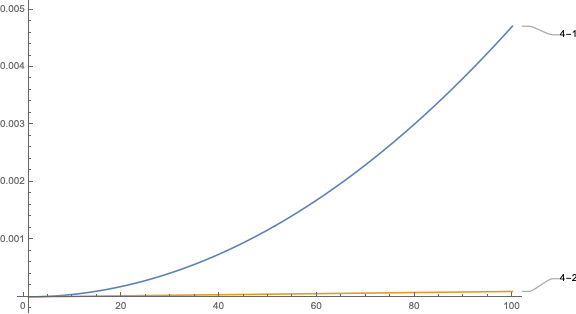
\includegraphics[width=4in]{source/4-4.png}
  \centering
\end{figure}
\small{*The formular used for plot is different than the actual (exponent reduced to 20 from 128).}

Similar as birthday paradox, the probability of finding two random string with same first 24 bits is larger than find a string has same first 24 bits. \\

4-1: Probability for finding two random strings with same first 24 bits (out of 128).
$$1-\frac{2^{128}!}{\left(2^{128}\right)^{n} \left(2^{128}-n\right)!}$$

4-2: Probability for finding a random string with same first 24 bits (out of 128) by given message.
$$1-\left(\frac{2^{128}-1}{2^{128}}\right)^{n}$$
\end{enumerate}

\section{Submitting Your Homework}
Please write a report describing how you solve each of the problem above, and submit at CARMEN.

\end{document}